\begin{frame}[fragile]{Polyhedral Enclosures}
    \begin{definition}[Polyhedral Enclosure]
        Let $ \mathcal{B} = \langle n,P, L, U \rangle $ be a bounding set, let $\Delta$ be a Delaunay triangulation of $P$, and let $\Delta_n$ be the set of all $n$-simplices in $\Delta$. We then define the bounding set associated with a simplex $\mathcal{S} \in \Delta_n$ as:
        \[
        \mathcal{B}_{\mathcal{S}} := \langle n,\mathbf{vert}(\mathcal{S}), L^{\mathbf{vert}(\mathcal{S})}, U^{\mathbf{vert}(\mathcal{S})} \rangle,
        \]
        \vspace{0.5em} 
        \noindent
        We define the \emph{polyhedral enclosure} formed by $\mathcal{B}$ and $\Delta$ as:
        \[
        \mathcal{E}(\mathcal{B},\Delta) := \bigcup_{S\in\Delta_n} \mathcal{P}(\mathcal{B}_S).
        \]
        \end{definition}
        
\end{frame}

\begin{frame}[fragile]{Polyhedral Enclosures}
    \begin{columns}
        \begin{column}{0.3\textwidth}
            \begin{definition}
                \[
                \mathcal{B}_{\mathcal{S}} := \langle n,\mathbf{vert}(\mathcal{S}), L^{\mathbf{vert}(\mathcal{S})}, U^{\mathbf{vert}(\mathcal{S})} \rangle,
                \]
                We define the \emph{polyhedral enclosure} formed by $\mathcal{B}$ and $\Delta$ as:
                \[
                \mathcal{E}(\mathcal{B},\Delta) := \bigcup_{S\in\Delta_n} \mathcal{P}(\mathcal{B}_S).
                \]
                \end{definition}
        \end{column}
        \begin{column}{0.6\textwidth}
            \begin{figure}
                \resizebox{0.7\columnwidth}{!}{
                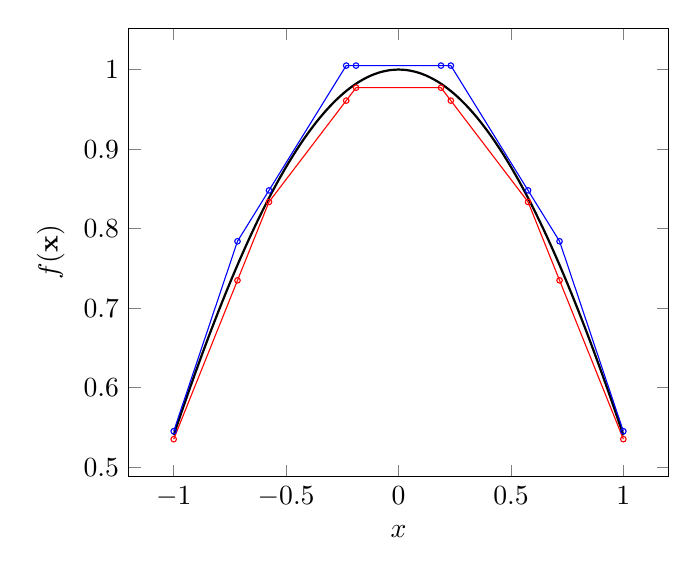
\begin{tikzpicture}
                    \begin{axis}[
                        name=plot1, % Name for referencing in arrows
                        xlabel={$x$},
                        ylabel={$f(\mathbf{x})$},
                        ]
                    
                        % Continuous plot
                        \addplot[color=black, thick, domain=-1:1, samples=1000] {cos(deg(x))};
                        
                        % Scatterplot 1
                        \addplot[color=red, mark=o, mark size=1pt] coordinates {
                        (-1.0, 0.5353023058681398)
                        (-0.7162290640736887, 0.7349957172856684)
                        (-0.5761808036482412, 0.8335495554233077)
                        (-0.23267298160795075, 0.9609732264310585)
                        (-0.18889649189051147, 0.9772120444891081)
                        (0.18889649189051147, 0.9772120444891081)
                        (0.23267298160795, 0.9609732264310588)
                        (0.5761808036482412, 0.8335495554233077)
                        (0.7162290640736885, 0.7349957172856686)
                        (1.0, 0.5353023058681398)
                        };
                        
                        % Scatterplot 2
                        \addplot[color=blue, mark=o, mark size=1pt] coordinates {
                        (-1.0, 0.5453023058681398)
                        (-0.7162290640736887, 0.7840873150595451)
                        (-0.5761808036482412, 0.8480683885144896)
                        (-0.23267298160795075, 1.005)
                        (-0.18889649189051147, 1.005)
                        (0.18889649189051147, 1.005)
                        (0.23267298160795, 1.005)
                        (0.5761808036482412, 0.8480683885144897)
                        (0.7162290640736885, 0.7840873150595453)
                        (1.0, 0.5453023058681398)
                        };
                    \end{axis}
                \end{tikzpicture}}
            \end{figure}
        \end{column}
    \end{columns}
\end{frame}

\begin{frame}[fragile]{Polyhedral Enclosures: Composition}
    \begin{definition}[Bounding Set Composition]
        Let $\mathcal{B}^f = \langle n, P, L^f, U^f \rangle$ and $\mathcal{B}^g = \langle n, P, L^g, U^g \rangle$ be bounding sets with the same dimension and over the same set of points $P$.  For $\bowtie\ \in\{+,-,\times,/\}$, we define $\mathcal{B}^f \bowtie \mathcal{B}^g := \langle n, P, L, U \rangle$, where, for all $\vec{x} \in P$,
            \begin{align*} 
            &L(\vec{x}), U(\vec{x}) = \\
            &\begin{cases}
                L^f(\vec{x}) + L^g(\vec{x}), U^f(\vec{x}) + U^g(\vec{x}) & \text{if } \bowtie \, = \,+, \\[0.1ex]
                L^f(\vec{x}) - L^g(\vec{x}), U^f(\vec{x}) - U^g(\vec{x}) & \text{if } \bowtie \, = \,-, \\[0.1ex]
                \min(\mathit{Bounds}),\max(\mathit{Bounds})  & \text{if } \bowtie \, \in \{\times, \div\}, \\[0.1ex]
            \end{cases}
            \end{align*}
            where $\mathit{Bounds} = \{h_1(x) \bowtie h_2(x) \,|\, h_1 \in \{L^f, U^f\}, h_2 \in \{L^g, U^g\} \}$ is the set of potential bounds when using multiplication or division.
        \end{definition}
        
\end{frame}

\begin{frame}[fragile]{Polyhedral Enclosures: Composition}
    \begin{figure}
        \resizebox{\textwidth}{!}{
        \begin{tikzpicture}
        % Tree Graph
        \node[anchor=north] (tree) at (-1cm, 1.5cm) {
            \begin{tikzpicture}[
                grow=down, % Tree grows to the right
                sibling distance=2cm, % Horizontal spacing between sibling nodes
                level distance=1cm, % Vertical spacing between parent and child
                edge from parent/.style={draw, -stealth}, % Arrow style for edges
                every node/.style={circle, draw, minimum size=1.5cm} % Default node style
            ]
                % Root node with its own style
                \node {$\otimes$}
                    % First child node with a different style
                    child {node {$\mathbf{x}_4$}}
                    % Second child node with another style
                    child {node {$\cos(\mathbf{x}_3)$}};
            \end{tikzpicture}
        };


        % Line Plot 1
        \begin{axis}[
            name=plot1, % Name for referencing in arrows
            at={(2cm,0)}, % Position
            width=5cm, % Width of the first plot
            height=4cm,
            xlabel={$x_3$},
            ylabel={$f(\mathbf{x}_3)$},
            legend style={at={(1.05,1.2)}, anchor=north west}, % Position legend outside plot
            legend cell align={left} % Align legend entries
        ]

        % Continuous plot
        \addplot[color=black, thick, domain=-1:1, samples=1000] {cos(deg(x))};
        \addlegendentry{$f(\mathbf{x}_3) = \cos(\mathbf{x}_3)$}

        % Scatterplot 1
        \addplot[color=red, mark=o, mark size=1pt] coordinates {
        (-1.0, 0.5353023058681398)
        (-0.7162290640736887, 0.7349957172856684)
        (-0.5761808036482412, 0.8335495554233077)
        (-0.23267298160795075, 0.9609732264310585)
        (-0.18889649189051147, 0.9772120444891081)
        (0.18889649189051147, 0.9772120444891081)
        (0.23267298160795, 0.9609732264310588)
        (0.5761808036482412, 0.8335495554233077)
        (0.7162290640736885, 0.7349957172856686)
        (1.0, 0.5353023058681398)
        };
        \addlegendentry{Lower Bounds}

        % Scatterplot 2
        \addplot[color=blue, mark=o, mark size=1pt] coordinates {
        (-1.0, 0.5453023058681398)
        (-0.7162290640736887, 0.7840873150595451)
        (-0.5761808036482412, 0.8480683885144896)
        (-0.23267298160795075, 1.005)
        (-0.18889649189051147, 1.005)
        (0.18889649189051147, 1.005)
        (0.23267298160795, 1.005)
        (0.5761808036482412, 0.8480683885144897)
        (0.7162290640736885, 0.7840873150595453)
        (1.0, 0.5453023058681398)
        };
        \addlegendentry{Upper Bounds}
        \end{axis}

        % Line Plot 2
        \begin{axis}[
            name=plot2, % Name for referencing in arrows
            at={(2cm,-4cm)}, % Position below the first plot
            width=5cm,
            height=4cm,
            xlabel={$x_4$},
            ylabel={$f(\mathbf{x}_4)$},
            legend style={at={(1.05,0.5)}, anchor=north west}, % Position legend outside plot
            legend cell align={left} % Align legend entries
        ]
        % Continuous plot
        \addplot[color=black, thick, domain=-1:1, samples=1000] {x};
        \addlegendentry{$f(\mathbf{x}_4) = \mathbf{x}_4$}

        % Scatterplot 1
        \addplot[color=red, mark=o, mark size=1pt] coordinates {
        (-1.0, -1.0500000000010001)
        (1.0, 0.949999999999)
        };
        \addlegendentry{Lower Bounds}

        % Scatterplot 2
        \addplot[color=blue, mark=o, mark size=1pt] coordinates {
        (-1.0, -0.949999999999)
        (1.0, 1.0500000000010001)
        };
        \addlegendentry{Upper Bounds}

        \end{axis}

        \begin{axis}[
            name=surface,
            at={(10.5cm,-1.9cm)}, % Position to the right of line plots
            width=7cm,
            view={30}{15}, % Viewing angle
            xlabel={$\mathbf{x}_3$},
            ylabel={$\mathbf{x}_4$},
            zlabel={$f(\mathbf{x})$},
            clip=false,
            legend style={
                at={(0.5,-0.25)}, % Position legend outside plot area
                anchor=north, % Align legend to this point
            }
        ]
        % Surface defined by specific points
        \addplot3[
            surf, mesh/rows=2,
            color=red,
            opacity = 0.5
        ] coordinates
        {
        (-1.0, -1.0, -0.5403023058766738)
        (-0.7162290640736887, -1.0, -0.8963621083899191)
        (-0.5761808036482412, -1.0, -0.8566248877968725)
        (-0.23267298160795075, -1.0, -1.1020803207157925)
        (-0.18889649189051147, -1.0, -1.0533638665416554)
        (0.18889649189051147, -1.0, -1.0533638665416554)
        (0.23267298160795, -1.0, -1.1020803207157925)
        (0.5761808036482412, -1.0, -0.8566248877968725)
        (0.7162290640736885, -1.0, -0.8963621083899191)
        (1.0, -1.0, -0.5403023058766738)
        (-1.0, 1.0, 0.5403023058595977)
        (-0.7162290640736887, 1.0, 0.5836293261814305)
        (-0.5761808036482412, 1.0, 0.820474223049743)
        (-0.23267298160795075, 1.0, 0.8298661321463285)
        (-0.18889649189051147, 1.0, 0.9110602224365536)
        (0.18889649189051147, 1.0, 0.9110602224365536)
        (0.23267298160795, 1.0, 0.8298661321463285)
        (0.5761808036482412, 1.0, 0.820474223049743)
        (0.7162290640736885, 1.0, 0.5836293261814305)
        (1.0, 1.0, 0.5403023058595977)
        };
        \addlegendentry{Lower Bounds}
        \addplot3[
            surf,  
            shader=flat,
            color=black,
            domain=-1:1, % Set x domain
            domain y=-1:1, % Set y domain
            samples=50, 
            opacity=0.5
        ] 
        {y*cos(deg(x))};
        \addlegendentry{$f(\mathbf{x}) = \mathbf{x}_4\cos(\mathbf{x}_3)$}

        Surface defined by specific points
        \addplot3[
            surf, mesh/rows=2,
            color=blue,
            opacity = 0.5
        ] 
        coordinates {
        (-1.0, -1.0, -0.5403023058595959)
        (-0.7162290640736887, -1.0, -0.62272092395526)
        (-0.5761808036482412, -1.0, -0.8249930561409187)
        (-0.23267298160795075, -1.0, -0.8638929057152325)
        (-0.18889649189051147, -1.0, -0.9288481779474296)
        (0.18889649189051147, -1.0, -0.9288481779474296)
        (0.23267298160795, -1.0, -0.8638929057152325)
        (0.5761808036482412, -1.0, -0.8249930561409187)
        (0.7162290640736885, -1.0, -0.62272092395526)
        (1.0, -1.0, -0.5403023058595959)
        (-1.0, 1.0, 0.5403023058766863)
        (-0.7162290640736887, 1.0, 0.9354537061638268)
        (-0.5761808036482412, 1.0, 0.8611437208880623)
        (-0.23267298160795075, 1.0, 1.1361070942847675)
        (-0.18889649189051147, 1.0, 1.0711518220525704)
        (0.18889649189051147, 1.0, 1.0711518220525704)
        (0.23267298160795, 1.0, 1.1361070942847675)
        (0.5761808036482412, 1.0, 0.8611437208880623)
        (0.7162290640736885, 1.0, 0.9354537061638268)
        (1.0, 1.0, 0.5403023058766863)
        };
        \addlegendentry{Upper Bounds}
        \end{axis}
        \end{tikzpicture}}
    \end{figure}
\end{frame}

\begin{frame}[fragile]{Polyhedral Enclosures}
    Polyhedral enclosures are \textbf{an efficient combinatorial abstraction} for nonlinear dynamical systems.
\end{frame}